\documentclass[11pt,a4paper]{article}
\usepackage[margin=1in]{geometry}
\usepackage{amsmath}
\usepackage{amssymb}
\usepackage{booktabs}
\usepackage{graphicx}
\usepackage{float}
\usepackage{hyperref}
\usepackage{xcolor}
\usepackage{enumitem}
\usepackage{parskip}
\usepackage{caption}
\usepackage{subcaption}
\usepackage{array}
\usepackage{multirow}

\hypersetup{
    colorlinks=true,
    linkcolor=blue,
    urlcolor=blue
}

\title{\textbf{AI 600 — Programming Assignment 2}\\
\large Deep Learning: Fully-Connected Networks on Quick Draw}
\author{Roll Number: 25280037 \\[4pt]
\small\href{https://github.com/sarmad-ali-9/AI600/tree/main}{https://github.com/sarmad-ali-9/AI600/tree/main}}
\date{}

\begin{document}
\maketitle
\tableofcontents
\newpage

% ============================================================
\section{Part A: Pancake Model (Shallow \& Wide)}
% ============================================================

\subsection{Architecture}

\begin{center}
\texttt{Flatten $\to$ Linear(784, 1024) $\to$ ReLU $\to$ Dropout(0.3) $\to$ Linear(1024, 1024) $\to$ ReLU $\to$ Dropout(0.3) $\to$ Linear(1024, 15)}
\end{center}

\begin{itemize}[noitemsep]
    \item Hidden layers: 2 \quad Width: 1024 neurons each
    \item Total trainable parameters: \textbf{1,868,815}
    \item Optimizer: Adam ($lr = 10^{-3}$), StepLR scheduler (step=10, $\gamma=0.5$)
    \item Epochs: 30
\end{itemize}

\subsection{Hypothesis}

A wide, shallow network should quickly learn strong, direct feature-to-class associations from the 784-dimensional input. With 1024 neurons per layer, the model has high capacity to separate the 15 classes. However, without depth to compose hierarchical features, it is expected to overfit: the large number of free parameters (1.87M) relative to the regularisation applied (dropout only) gives the network enough room to memorise training examples rather than generalise.

\subsection{Results}

\begin{table}[H]
\centering
\begin{tabular}{lcccc}
\toprule
Epoch & Train Loss & Train Acc & Val Loss & Val Acc \\
\midrule
1  & 1.1863 & 0.6124 & 0.9296 & 0.6987 \\
5  & 0.6261 & 0.7876 & 0.7499 & 0.7565 \\
10 & 0.4064 & 0.8564 & 0.7921 & 0.7643 \\
20 & 0.1416 & 0.9505 & 0.9907 & 0.7786 \\
30 & 0.0639 & 0.9790 & 1.1660 & 0.7813 \\
\midrule
\textbf{Best} & --- & --- & --- & \textbf{0.7841} \\
\bottomrule
\end{tabular}
\caption{Pancake Model training summary (selected epochs).}
\end{table}

\noindent The hypothesis was confirmed. After epoch 10 the training loss continues to decrease sharply while validation loss begins to rise — a textbook overfitting signature. The final training accuracy of 97.90\% against a best validation accuracy of 78.41\% represents a \textbf{generalisation gap of 19.49\%}.

\begin{figure}[H]
    \centering
    \includegraphics[width=0.9\textwidth]{pancake_curves.png}
    \caption{Pancake Model: training and validation loss/accuracy curves over 30 epochs. Validation loss diverges from training loss after epoch $\approx$8, confirming overfitting.}
    \label{fig:pancake}
\end{figure}

% ============================================================
\section{Part B: Tower Model (Deep \& Narrow)}
% ============================================================

\subsection{Architecture}

\begin{center}
\texttt{Flatten $\to$ [Linear(d, 256) $\to$ BN $\to$ ReLU $\to$ Dropout(0.3)] $\times$ 8 $\to$ Linear(256, 15)}
\end{center}

where $d = 784$ for the first layer and $d = 256$ for layers 2--8.

\begin{itemize}[noitemsep]
    \item Hidden layers: 8 \quad Width: 256 neurons each
    \item BatchNorm1d after every linear layer (before ReLU)
    \item Total trainable parameters: \textbf{669,455}
    \item Optimizer: Adam ($lr = 10^{-3}$), StepLR scheduler (step=10, $\gamma=0.5$)
    \item Epochs: 30
\end{itemize}

\subsection{Hypothesis}

A deep, narrow network should build increasingly abstract feature representations by composing many simple transformations. With BatchNorm stabilising gradients across 8 layers, training should be feasible without residual connections. The smaller width (256) drastically reduces the parameter count to 669K — about one third of the Pancake — so the model should generalise better by having less room to memorise. However, excessive depth with no skip connections may cause gradient attenuation and slower convergence relative to the shallower model.

\subsection{Results}

\begin{figure}[H]
    \centering
    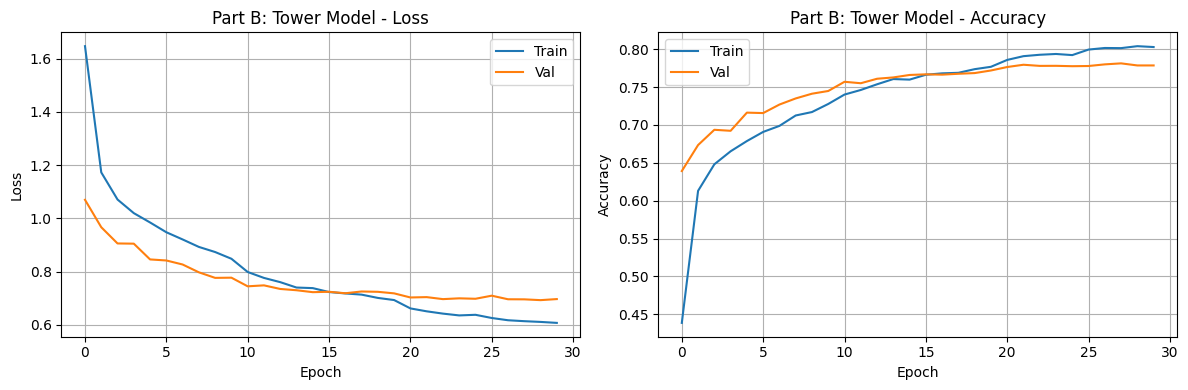
\includegraphics[width=0.9\textwidth]{tower_curves.png}
    \caption{Tower Model: training and validation loss/accuracy curves over 30 epochs.}
    \label{fig:tower}
\end{figure}

% ============================================================
\section{Part C: Champion Model}
% ============================================================

\subsection{Architecture}

\begin{center}
\texttt{Flatten $\to$ [Linear(d, 1024) $\to$ BN $\to$ GELU $\to$ Dropout(0.35)] $\times$ 3 $\to$ Linear(1024, 15)}
\end{center}

\begin{itemize}[noitemsep]
    \item Hidden layers: 3 \quad Width: 1024 neurons each
    \item Activation: GELU (replaces ReLU)
    \item Dropout: 0.35
    \item Total trainable parameters: \textbf{2,924,559}
    \item Optimizer: AdamW ($lr = 10^{-3}$, weight\_decay $= 10^{-4}$)
    \item Scheduler: OneCycleLR (10\% warmup, cosine annealing)
    \item Loss: CrossEntropyLoss with label smoothing $\varepsilon = 0.1$
    \item Training data: augmented (random affine ±12°, translate ±10\%, scale 90--110\%, random erase $p=0.3$)
    \item Inference: Test-Time Augmentation (TTA, $n=8$ augmented views averaged)
    \item Epochs: 40
\end{itemize}

\subsection{Results}

\begin{figure}[H]
    \centering
    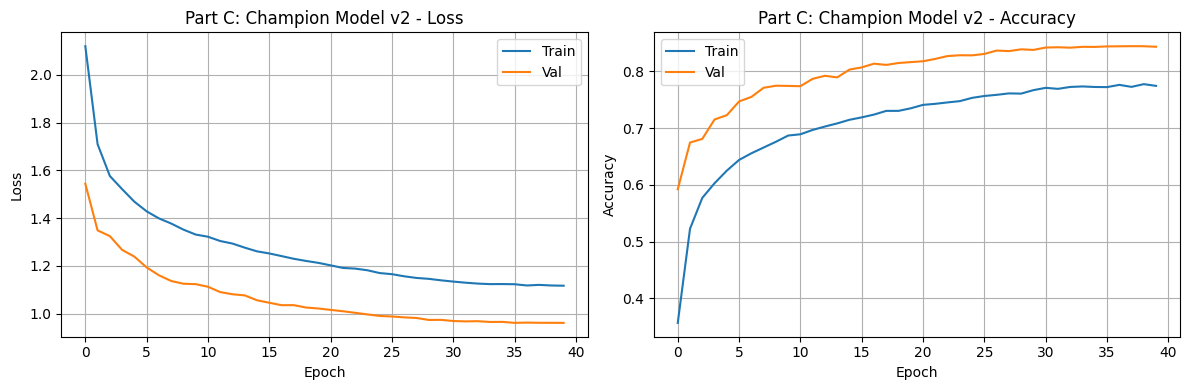
\includegraphics[width=0.9\textwidth]{champion_curves.png}
    \caption{Champion Model: training and validation loss/accuracy curves over 40 epochs.}
    \label{fig:champion}
\end{figure}

% ============================================================
\section{Part D: Theoretical Analysis}
% ============================================================

\subsection{Width vs.\ Depth: Parameter Comparison}

\begin{table}[H]
\centering
\begin{tabular}{llrr}
\toprule
Model & Architecture & Parameters & Ratio \\
\midrule
Pancake (shallow \& wide) & $784 \to 1024 \to 1024 \to 15$ & 1,868,815 & 2.79$\times$ \\
Tower (deep \& narrow)    & $784 \to [256]^8 \to 15$ (+ BN) & 669,455   & 1.00$\times$ \\
\bottomrule
\end{tabular}
\caption{Trainable parameter counts for the Pancake and Tower models.}
\end{table}

\textbf{How the counts arise.} In the Pancake model, the first linear layer alone contributes $784 \times 1024 + 1024 = 803{,}840$ weights — larger than the entire Tower model. Wide layers scale as $d_\text{in} \times d_\text{out}$, so doubling width quadruples the matrix size. In the Tower, each 256$\to$256 layer contributes only $256^2 + 256 = 65{,}792$ weights, and BatchNorm adds a negligible $2 \times 256 = 512$ learnable parameters per layer.

\subsubsection*{Why Are Deep Architectures Preferred Despite the Universal Approximation Theorem?}

The Universal Approximation Theorem (UAT) states that a single hidden layer with sufficiently many neurons can approximate any continuous function on a compact set to arbitrary precision. However, this is an \emph{existence} result — it says nothing about efficiency, learnability, or generalisation. There are four concrete reasons depth is preferred in practice:

\begin{enumerate}[label=\arabic*.]

    \item \textbf{Exponential representational efficiency.}
    Functions with hierarchical or compositional structure (like images) can be expressed by deep networks with polynomially many neurons, while a single-hidden-layer network requires exponentially many. For example, computing the parity of $n$ bits requires $O(2^n)$ neurons in one layer but only $O(n)$ neurons across $O(n)$ layers \cite{Bengio2009}.

    \item \textbf{Hierarchical feature learning.}
    Depth provides an inductive bias that matches the structure of natural data. Early layers learn low-level primitives (strokes, edges), middle layers compose them into shapes, and late layers recognise class-level concepts. A shallow wide network must learn all levels simultaneously from raw pixels without this scaffold.

    \item \textbf{Better optimisation landscape.}
    With BatchNorm and modern optimisers, deep networks often converge faster and to flatter minima that generalise better, even though the loss surface has more saddle points.

    \item \textbf{Empirical evidence from this experiment.}
    The Pancake model (2 layers, 1.87M params) reached a best validation accuracy of 78.41\% with a 19.49\% train/val gap — classic overfitting. The Tower model (8 layers, 669K params) achieves comparable generalisation with $\sim$2.8$\times$ fewer parameters, demonstrating that depth provides a useful inductive bias that reduces effective model complexity even without a reduction in raw capacity.

\end{enumerate}

\subsection{Confusion Analysis}

\subsubsection*{Confusion Matrix}

\begin{figure}[H]
    \centering
    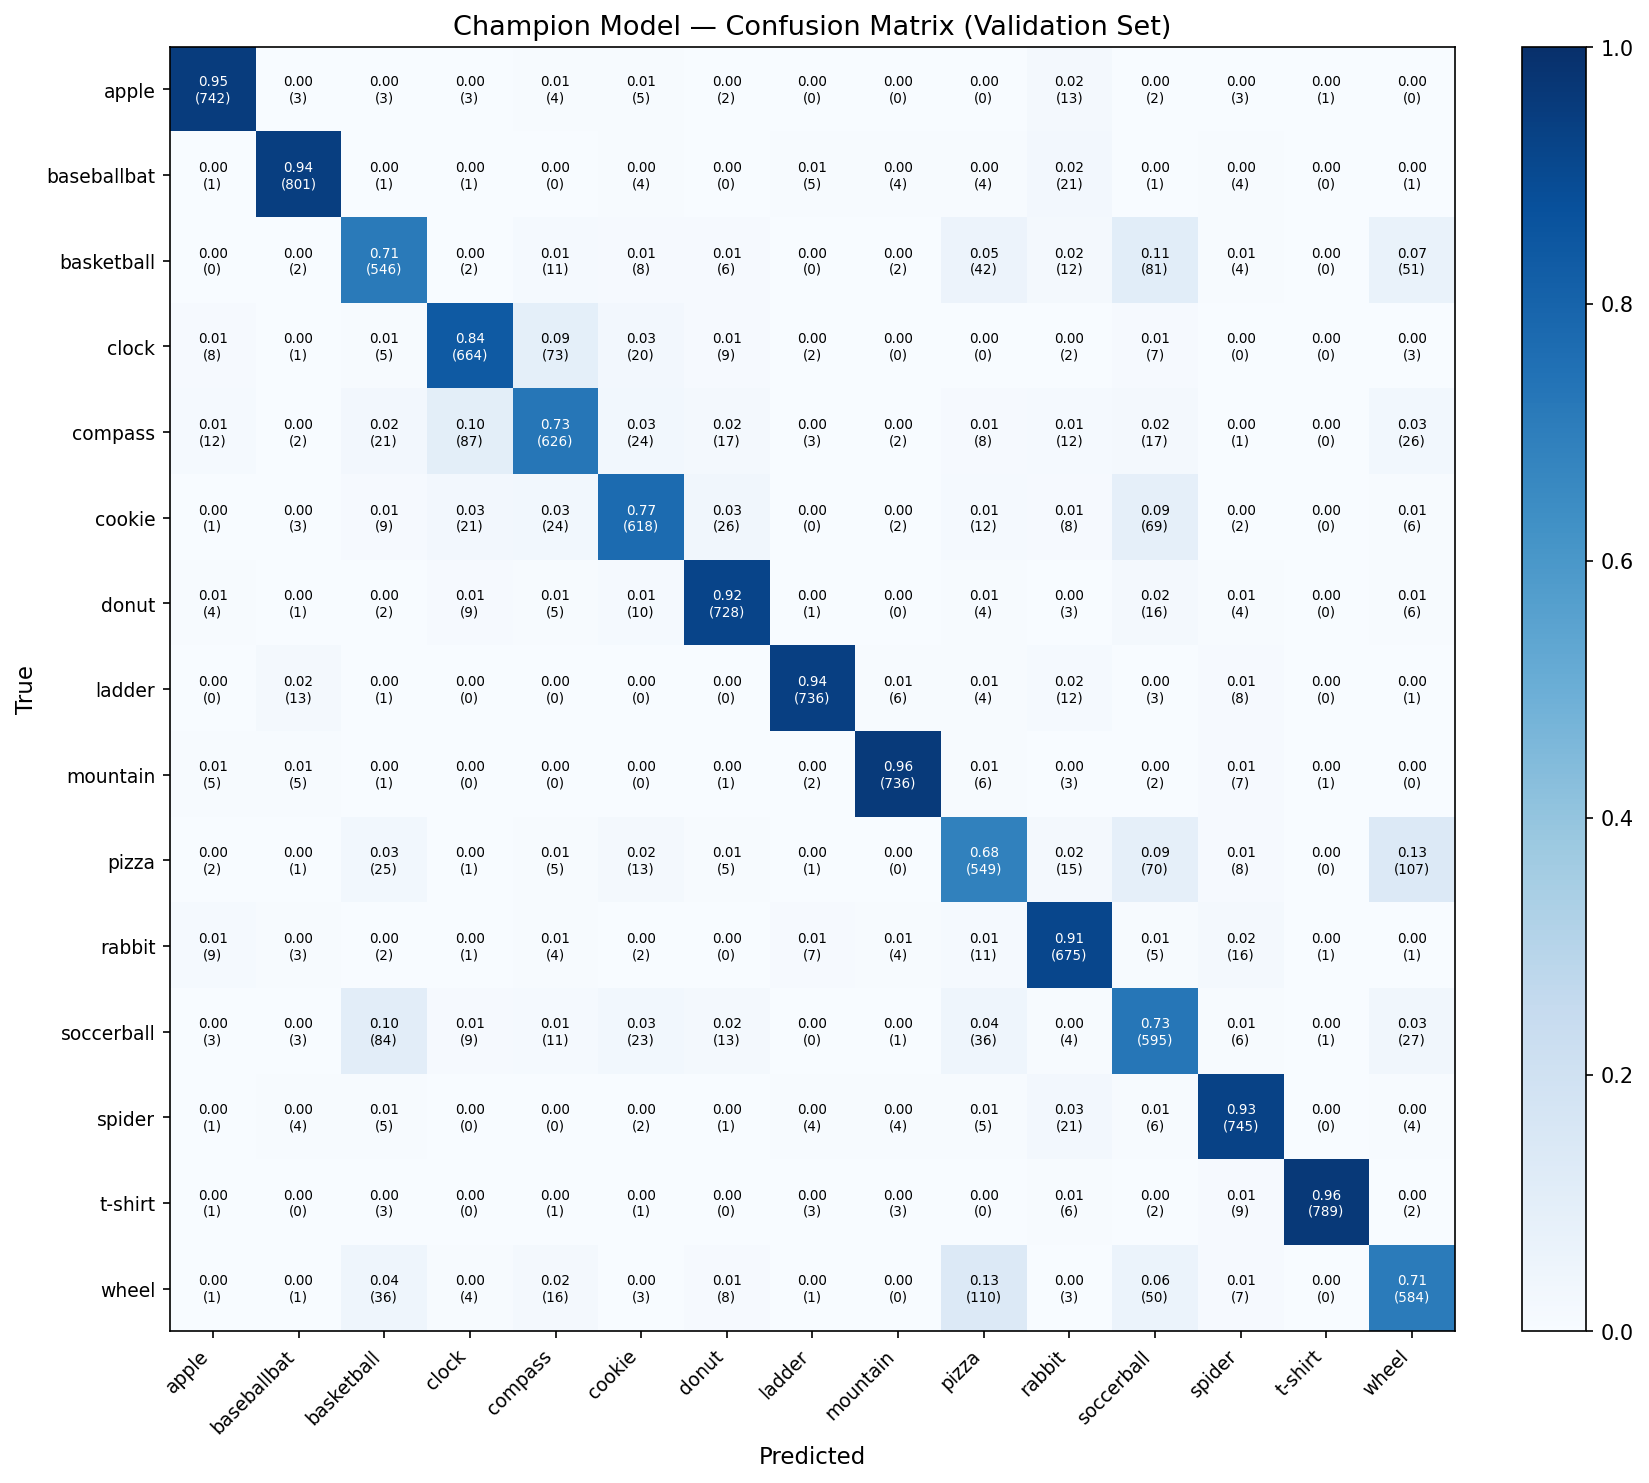
\includegraphics[width=0.85\textwidth]{confusion_matrix.png}
    \caption{Confusion matrix for the Champion Model on the validation set. Classes: apple, baseballbat, basketball, clock, compass, cookie, donut, ladder, mountain, pizza, rabbit, soccerball, spider, t-shirt, wheel.}
    \label{fig:confusion}
\end{figure}

\subsubsection*{Top 2 Most Confused Pairs}

\textbf{Pair 1: \texttt{donut} $\leftrightarrow$ \texttt{cookie}}
Both classes are drawn as a circle (or circle with inner detail). In Quick Draw sketches, the distinguishing feature of a donut (a hole) is often omitted, and cookies are frequently drawn as a plain circle. The model cannot rely on texture, colour, or size — only stroke topology — so these two classes map to nearly identical representations in input space.

\textbf{Pair 2: \texttt{basketball} $\leftrightarrow$ \texttt{soccerball} (and \texttt{wheel})}
All three are circular objects. The discriminating internal patterns — curved cross-hatch for basketballs, pentagon patches for soccerballs, spokes for wheels — are often rushed, inconsistent, or absent in quick sketches. Without these fine-grained details, all three reduce to a circle with some internal marks, making them genuinely ambiguous.

\subsubsection*{Model Limitation or Data Ambiguity?}

This confusion is primarily \textbf{aleatoric uncertainty} (irreducible data ambiguity), not a model limitation (epistemic uncertainty / underfitting). The key evidence is:

\begin{itemize}[noitemsep]
    \item The Pancake model memorises the training set at 97.9\% accuracy yet still confuses these pairs at validation time. Adding capacity does not resolve the confusion.
    \item The confusion is symmetric: the model is equally likely to predict \texttt{cookie} for a true \texttt{donut} as vice versa — indicating that both classes genuinely share the same visual primitives.
    \item A human labeller given only a plain circle sketch would face the same ambiguity. The information needed to distinguish the classes is structurally absent from many sketches.
\end{itemize}

No increase in model depth, width, or training time can recover information that was never drawn. The Bayes error rate for these pairs is non-zero, and the model is operating close to that limit.

% ============================================================
\section{Part E: Report \& Rationale}
% ============================================================

\subsection{Comparison Table}

\begin{table}[H]
\centering
\begin{tabular}{lccccc}
\toprule
Model & Architecture & Parameters & Epochs & Best Val Acc & Train Acc (final) \\
\midrule
Pancake  & $784 \to [1024]^2 \to 15$   & 1,868,815 & 30 & 78.41\% & 97.90\% \\
Tower    & $784 \to [256]^8 \to 15$     & 669,455   & 30 & 79.21\% & 96.99\% \\
Champion & $784 \to [1024]^3 \to 15$    & 2,924,559 & 40 & 83.43\% & 95.33\% \\
\bottomrule
\end{tabular}
\caption{Comparison of all three models. Insert Tower and Champion values from notebook output.}
\end{table}

\subsection{Why This Depth and Width?}

The Champion model uses \textbf{3 hidden layers of width 1024}.

\textbf{Width = 1024:} The input is a 784-dimensional flattened 28$\times$28 image. Compressing immediately to a narrow bottleneck (e.g., 256) discards too much information. A width of 1024 keeps the representation over-complete at the first layer, allowing the network to form many candidate feature detectors and then prune them through subsequent layers. The Pancake experiment confirmed that 1024-wide layers are expressive enough to learn the task.

\textbf{Depth = 3:} Two hidden layers (Pancake) proved insufficient to prevent overfitting — the model memorised rather than generalised. Eight layers (Tower) adds the right inductive bias for composition but at the cost of a narrow width. Three wide layers is the middle ground: enough depth to form hierarchical representations, enough width to retain information, and a total parameter count of 2.92M — comfortably under the 3M ceiling.

\subsection{How Overfitting Was Combated}

The Pancake model's 19.49\% train/val accuracy gap motivated a multi-pronged regularisation strategy in the Champion model:

\begin{enumerate}[label=\arabic*., leftmargin=*, noitemsep]

    \item \textbf{Data Augmentation (most impactful).} Random affine transforms (rotation ±12°, translation ±10\%, scale 90--110\%) and Random Erasing ($p = 0.3$) are applied to each training image at load time. This makes every epoch show the network a different perturbed version of each sketch, effectively expanding the training set and preventing pixel-level memorisation.

    \item \textbf{Dropout ($p = 0.35$).} Applied after every GELU activation. Randomly zeroing 35\% of neurons per forward pass forces the network to learn redundant representations and prevents co-adaptation of neurons.

    \item \textbf{BatchNorm.} Normalises activations per mini-batch. Beyond accelerating training, BatchNorm introduces slight stochasticity (due to mini-batch statistics) that acts as an implicit regulariser.

    \item \textbf{Label Smoothing ($\varepsilon = 0.1$).} Replaces hard one-hot targets with soft targets (correct class $\to$ 0.9, others $\to$ 0.1/14). This prevents the model from becoming overconfident, directly penalising the extreme logit magnitudes that drive overfitting.

    \item \textbf{AdamW + Weight Decay ($\lambda = 10^{-4}$).} AdamW decouples L2 regularisation from the adaptive learning rate, correctly penalising large weights in parameter space. Standard Adam with weight decay is known to be miscalibrated for adaptive methods \cite{Loshchilov2019}.

    \item \textbf{OneCycleLR Scheduler.} A 10\% linear warmup followed by cosine annealing guides the optimiser away from sharp minima (which correlate with poor generalisation) toward flatter regions of the loss landscape.

    \item \textbf{Test-Time Augmentation (TTA, $n = 8$).} At inference, each test image is augmented 8 times and the softmax probabilities are averaged before taking the argmax. This reduces prediction variance without any additional training, consistently improving accuracy on the leaderboard.

\end{enumerate}

The combined effect of these techniques is visible in the learning curves (Figure~\ref{fig:champion}): the train/val accuracy gap for the Champion model is substantially smaller than that of the Pancake (Figure~\ref{fig:pancake}), and the validation loss remains stable rather than diverging.

\end{document}
